%%% Copyright (C) 2004 Claire M. Connelly and 
%%% the Department of Mathematics, Harvey Mudd College.
%%%
%%% This file is part of the sample thesis document provided to HMC
%%% mathematics students.
%%%
%%% See the COPYING document, which should accompany this
%%% distribution, for information about distribution and modification
%%% of the document and its components.

\chapter{Resources}

There are lots of great resources available for using \tex and \latex.
Here are a few (there are also links available online at\\
\url{http://www.math.hmc.edu/computing/support/tex/}).


\section{Online Documentation}%
\label{sec:online-docs}

Much of the documentation for \tex and \latex is available online, as
part of the \tex system.  te\tex, the \tex system installed on the
mathematics department's computers, includes a script called
\prog{texdoc} to access this documentation.  All you have to do is
type \prog{texdoc} followed by a string that you believe is the name
of the document you're looking for.  For example, \prog{texdoc
  booktabs} will give you the documentation for the \package{booktabs}
package that I used to create the tables in this document.

Unfortunately, \prog{texdoc} only works for documentation that is
sensibly named.  The authors of the \package{graphics} package, for
instance, called their manual \file{grfguide}.  Still others decided
that \file{manual} was a good name for their manual (after all, it's
the only \emph{manual} in their distribution).

Sometimes you can find documentation using the \prog{locate} command,
which lists all the files on your system that match a string that you
provide.  For example, you could find \file{grfguide} by trying
\prog{locate graphics} and \prog{grep}ping out the results with
\file{texmf} in them, and passing that list to another \prog{grep} for
the string \file{doc}:
\begin{quote}
\begin{verbatim}
unix% locate graphics | grep texmf | grep doc
\end{verbatim}
\end{quote}

Another hard to find, but very useful, document, is the ``User's Guide
for the \package{amsmath} Package'' \citeyearpar{amsmath-doc}, which
is called \file{amsldoc}.

\subsection{\protect\command{texdoctk}}

Our current te\tex installation includes the \prog{texdoctk} program,
which gives you a graphical window into the documentation installed on
the system.  You start \prog{texdoctk} by typing its name at a shell
prompt.  A window (Figure~\ref{fig:texdoctk}) will appear with buttons
corresponding to broad categories of documentation; clicking on one
will open another dialog box with the titles of available
documentation (with the names of the actual packages in parentheses).

\begin{figure}[htbp]
  \centering
  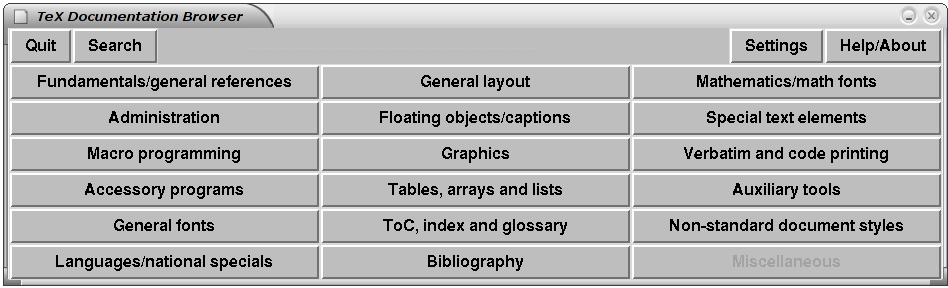
\includegraphics[width=\textwidth-2cm,keepaspectratio=true]{texdoctk}
  \caption[\protect\prog{texdoctk} main window]{\prog{texdoctk} main window.}
  \label{fig:texdoctk}
\end{figure}


\section{UK-TUG FAQ}

The primary list of frequently asked questions in the \tex world is
the UK TUG FAQ, available at
\url{http://www.tex.ac.uk/cgi-bin/texfaq2html}.  If you're not sure
how to do something, or you've got a problem that you're pretty sure
isn't being caused by a typo, check here first.


\section{\ctt}

If you can't find an answer in the UK-TUG FAQ, then your next step is
to check \ctt, the Usenet newsgroup devoted to \tex and \latex.
Chances are, whatever your problem is, someone else already had it,
asked about it on \texttt{c.t.t}, and got an answer.  Thanks to Google, Usenet's
past is preserved in an easily searchable format.  Go to Google Groups
(\url{http://groups.google.com/}), type in some search terms, and
check out the answers.  (If you specify \texttt{group:comp.text.tex}
at the end of your search terms, you'll only see results from \ctt.)


%%% Local Variables: 
%%% mode: latex
%%% TeX-master: "master"
%%% End: 
